\begin{figure*}[t]
    \centering
    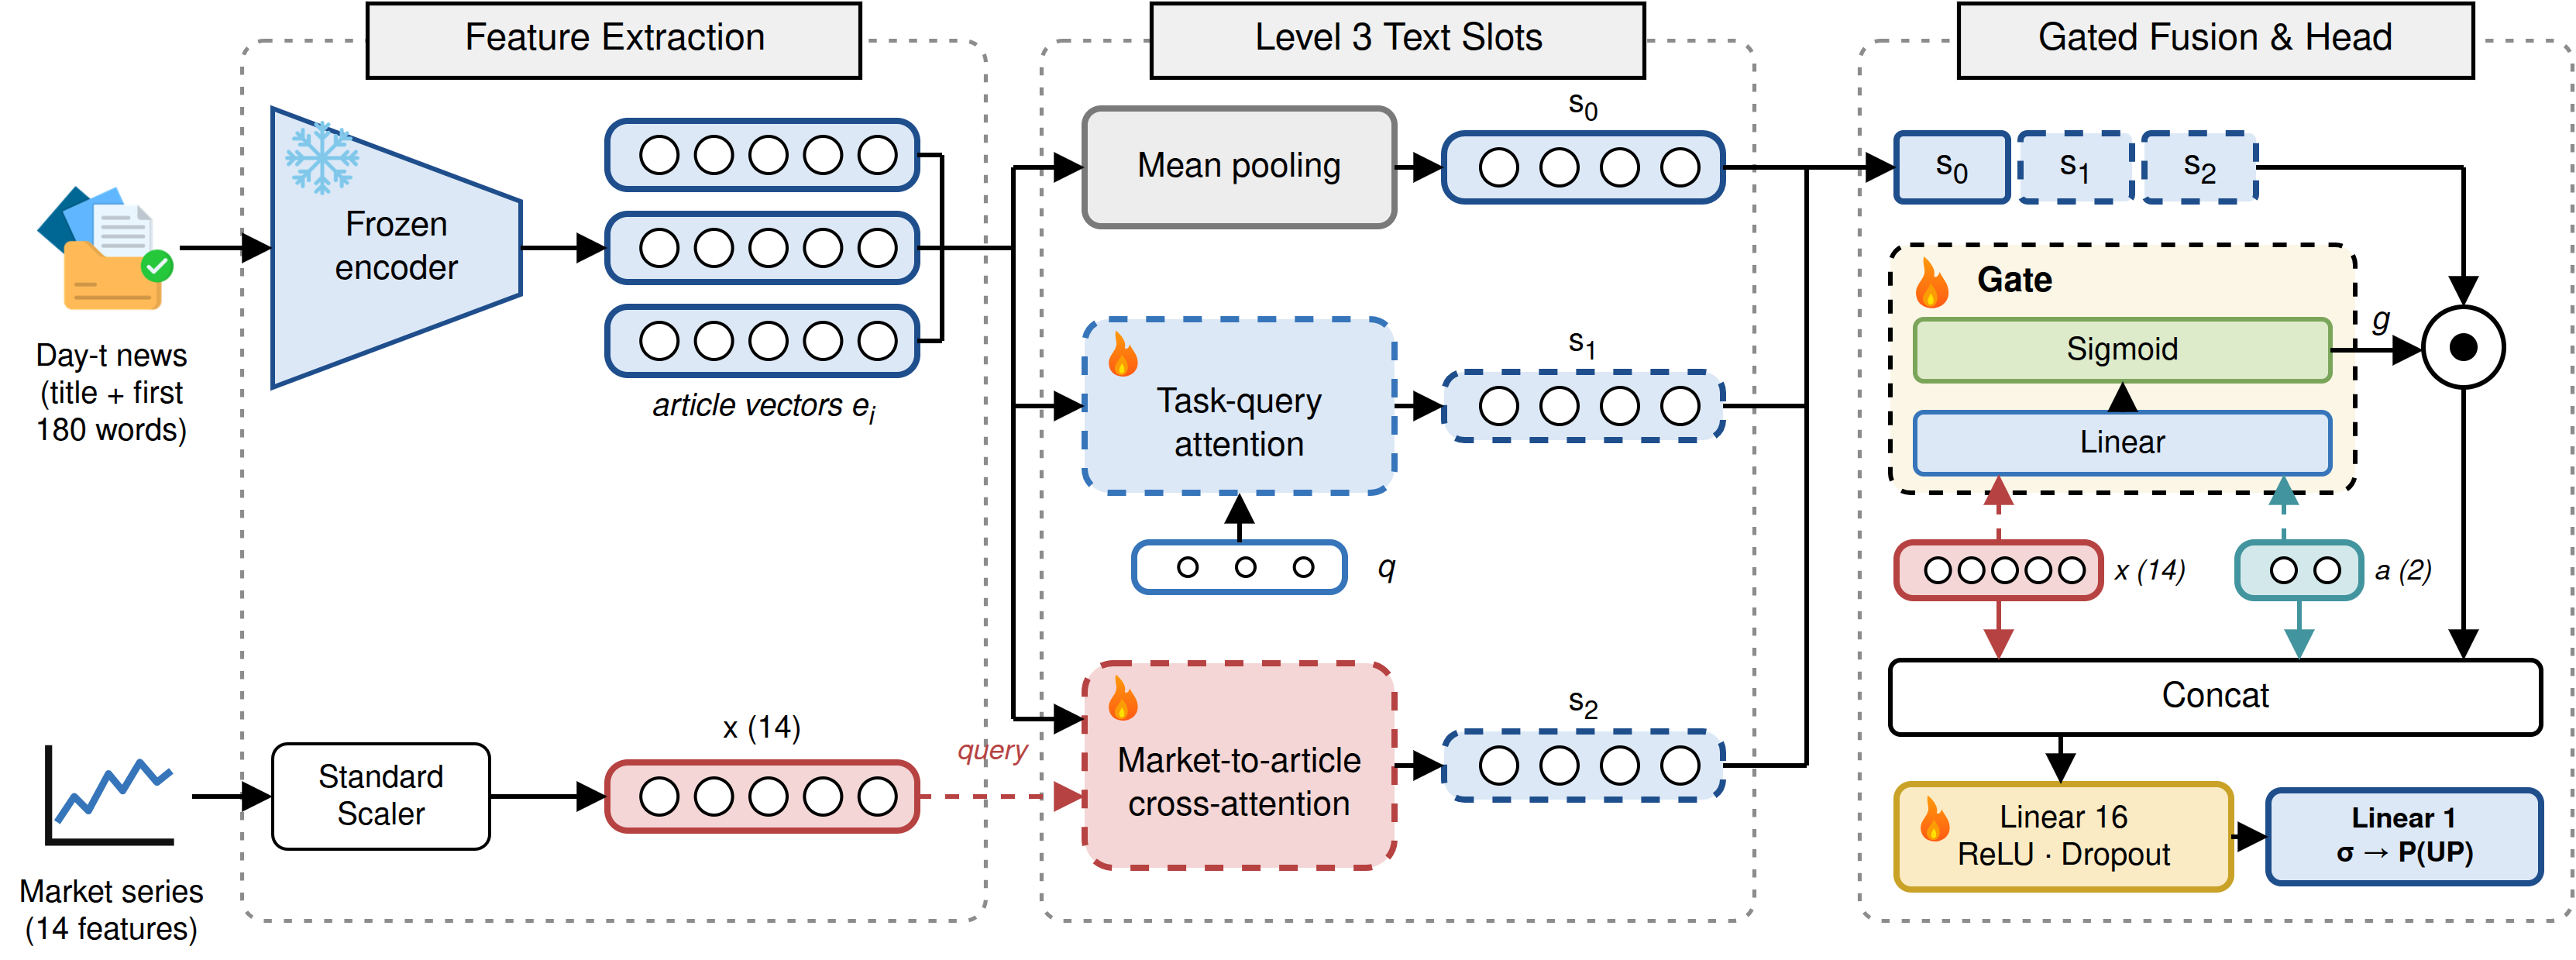
\includegraphics[width=\textwidth]{model_architecture.png}
    \caption{Level~3 architecture. A frozen encoder gives a 768-dimensional vector $\mathbf{e}_i$ per article. The mean slot $\mathbf{s}_0$ is always on. Dashed components switch on in addition to it: the task-query slot $\mathbf{s}_1$, the cross-attention slot $\mathbf{s}_2$, and the scalar gate. Slots are concatenated, and inactive slots are zero vectors. The gate reads the 14 market inputs $\mathbf{x}$ and the log article count, the first availability input, and $\odot$ scales all slots by the gate value $g$. $\mathbf{x}$ and both availability inputs $\mathbf{a}$ also join the concatenation. Flames mark trained parts and the snowflake marks the frozen encoder.}
    \label{fig:architecture}
\end{figure*}
